% to sort

% need plane direct diagram inkscape
% sphere coord needs middlie red line to get slice count consistent
% torus diagram needs colour
% fig refs not working ?
% code snipped links
% degenerate points




\documentclass[12pt,a4paper]{article}
\usepackage{graphicx}
\usepackage{hyperref}   
\usepackage{braket}
\usepackage{amsmath}

\usepackage[utf8]{inputenc}
\usepackage[english]{babel}

\usepackage{listings}
\usepackage{color}
\usepackage[margin=0.75in]{geometry}

\definecolor{mygreen}{rgb}{0,0.6,0}
\definecolor{mygray}{rgb}{0.5,0.5,0.5}
\definecolor{mymauve}{rgb}{0.58,0,0.82}
\usepackage{afterpage}
\usepackage{subcaption} 

\newcommand{\ts}{\textsuperscript}
\usepackage[super]{nth}
\usepackage{gensymb}
\usepackage{xcolor}
\usepackage{wasysym}
%\usepackage{wasysym} %for astro symbols

 \lstset{ 
  backgroundcolor=\color{white},  % choose the background color; you must add \usepackage{color} or \usepackage{xcolor}; should come as last argument
  basicstyle=\footnotesize,             % the size of the fonts that are used for the code
  breakatwhitespace=false,            % sets if automatic breaks should only happen at whitespace
  breaklines=true,                          % sets automatic line breaking
  captionpos=b,                             % sets the caption-position to bottom
  commentstyle=\color{mygreen},   % comment style
  deletekeywords={...},                   % if you want to delete keywords from the given language
  escapeinside={\%*}{*)},             % if you want to add LaTeX within your code
  extendedchars=true,                    % lets you use non-ASCII characters; for 8-bits encodings only, does not work with UTF-8
  frame=single,	                            % adds a frame around the code
  keepspaces=true,                         % keeps spaces in text, useful for keeping indentation of code (possibly needs columns=flexible)
  keywordstyle=\color{blue},            % keyword style
  language=Octave,                         % the language of the code
  morekeywords={*,...},                  % if you want to add more keywords to the set
  numbers=left,                               % where to put the line-numbers; possible values are (none, left, right)
  numbersep=5pt,                            % how far the line-numbers are from the code
  numberstyle=\tiny\color{mygray},   % the style that is used for the line-numbers
  rulecolor=\color{black},                 % if not set, the frame-color may be changed on line-breaks within not-black text (e.g. comments (green here))
  showspaces=false,                        % show spaces everywhere adding particular underscores; it overrides 'showstringspaces'
  showstringspaces=false,               % underline spaces within strings only
  showtabs=false,                           % show tabs within strings adding particular underscores
  stepnumber=2,                             % the step between two line-numbers. If it's 1, each line will be numbered
  stringstyle=\color{mymauve},        % string literal style
  tabsize=2,	                             % sets default tabsize to 2 spaces
  title=\lstname                               % show the filename of files included with \lstinputlisting; also try caption instead of title
} 

\usepackage[font=small,labelfont=bf]{caption} % Makes the font for figure captions smaller and the figure label bold.

\begin{document}
%\pagecolor{black}\afterpage{\nopagecolor}
%\color{white}
\begin{titlepage}
	\centering
	
\includegraphics[width=0.4\textwidth]{Images//Logos//rhul.jpg}\par\vspace{1cm}


	{\scshape\LARGE Royal Holloway University of London \par}
	\vspace{1cm}
	{\scshape\Large PH4100: Major Project\par}
	\vspace{1.5cm}
	{\huge\bfseries Meshing of Primitive Solids\\
	in\\
	pyg4ometry \& BDSIM\par}
	\vspace{2cm}
	{\Large\itshape Ben Shellswell\par}
	\vfill

\begin{abstract}
\centering

\end{abstract}

	\vfill
	
	Supervised by\par
	Prof.~S \textsc{Boogert} 

% Bottom of the page
	{\large \today\par}


\includegraphics[width=0.3\textwidth]{Images//Logos//BDSIM_Logo.jpg}\par\vspace{1cm}

\includegraphics[width=0.3\textwidth]{Images//Logos//JAI_Logo.jpeg}\par\vspace{1cm}

\end{titlepage}
\leavevmode\thispagestyle{empty}\newpage
%\color{black}
\tableofcontents
\thispagestyle{empty}
\newpage
\onecolumn

%%%%%%%%%%%%%%%%%%%%%%%%%%%%%%%%%%%%%%%%%%%%%%%%%%%%%%%%%%%%%%%%%%%%%%
\small
\setcounter{page}{1}
\section{Introduction}

\subsection{BDSIM}
BDSIM (or Beam Delivery SIMulation) is a software package written by the John Adams Institute for accelerator science (JAI), for the use of modelling particle beam interactions. BDSIM has many applications, such as modelling complex particle accelerators for example the Large Hadron Collider (LHC) and concepts magnets for MRI medical scanners.  

\subsection{pyg4ometry}
pyg4ometry is a python packaged also generated by JAI, its purpose it to convert 3D CAD models between different representations to allow compatibility with BDSIM for the testing of new concepts. The '4' in 'pyg4ometry' comes from the consistencey the package has with Geant4 \ref{geant4}.

\subsection{Geant4}\label{geant4}
Geant4 (or GEometry ANd Tracking) is a software developed for the simulation and tracking of particles traveling through matter.

\subsection{Project Aims}
The aims of this project are to optimize the pyg4ometry package to improve and performance test the results. The main areas for improvement and where most of the computational energy in wasted is in the meshing of the primitive Geant4 solids.

\section{Primitive Meshing}
This section will describe the work done to optimize the python scripts that generate the three dimensional meshing for the primitive solids. All the solids used are constructed such that they are compatible with Geant4's solids. It was orginally thought that it would be best to use triangles meshes to construct the 3D solids, however it has been realised that the computation of triangles compared with polygons is much more intensive and ineffecient, in most cases. In particular with the curved solids, i.e circular and elliptical based solids.
\\\\
All the python meshing scripts follow a similar structure of first defining an empty list of faces (polygons). Then running the associated trigonometric equations through a number of loops to generate and append polygons to that list. The number of loops is associated with the number of sections a surface of a solid is being split up into in a given coordinate system. The density of the meshing is defined by a user inputted number of slices and stacks, demonstrated in Figure \ref{cylcmeshin}

\subsection{Co-ordinate Systems}
The various primitive solids are all constructed by using the predefined paramters used by Geant4, to be consistent with Geant4's own solids. The parameters would be properties of a 3D solid such as height or radius. Which are then used as a way to define the points of the object via basic trigonometry.\

\subsubsection{Cylindrical Co-ordinate System}
The meshing for the primitive solids in cylindrical coordinate systems are constructed by looping though the number of slices and stacks which the cylinder is being cut into. The Loop then creates the coordinates for 3 or 4 points at a time, which can then be defined as a triangular or polygonal face. The only cases where the mesh produces triangles is at the top and bottom faces of the cylinder, provided it does has a minimum radius equal to zero (creating a tube or cone). 
%one on each slice as shown in Listing \ref{loopcode1} 

\begin{figure}[h!]
\centering
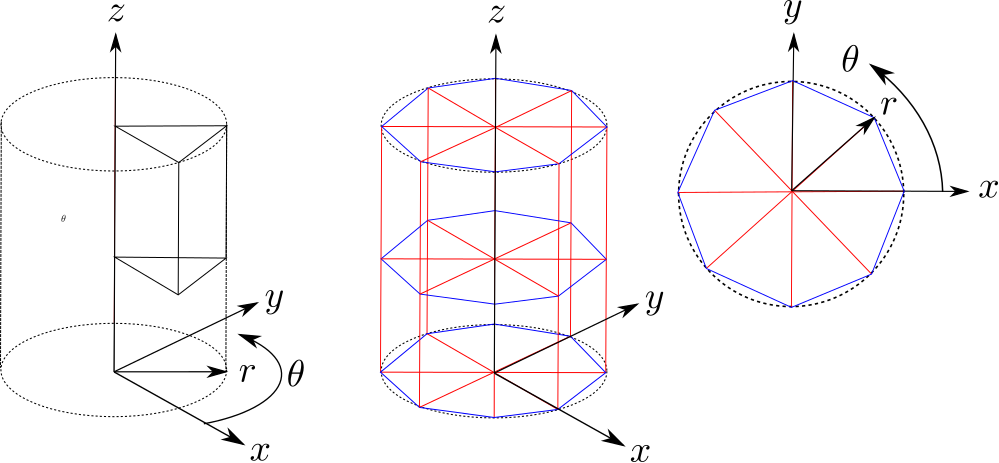
\includegraphics[scale=0.5]{Images//Coords//cyl.png}
\caption[width=\columnwidth]{Diagram showing the meshing method for a cylindrical coordinate system\\
Red = Slices (8)\\
Blue = Stack (2)}
\label{cylmeshin}
\end{figure}

The trigonometry that converts the points from cylindrical polar coordinates to cartesian, are:
\begin{equation}
\begin{split}
x = r \cos{\theta} \\
y = r \sin{\theta} \\
z = z
\end{split}
\end{equation}

\label{loopcode1} 
\begin{lstlisting}[language=Python, caption=Python example]
polygons = []

for j0 in range(nslice):
    j1 = j0
    j2 = j0 + 1
    
    vertices = []

    for i0 in range(nstack):
          i1 = i0
          i2 = i0 + 1     

\end{lstlisting}
The code in Listing \ref{loopcode1} generates counters so that you can choses from two slices and two stacks, in order to gain the four points surrounding a desired face. These points are then used to define a polygon. Same logic applies for the triangles, just using 3 points.
\\\\
The only time stack is needed in the cylindrical coordinate system is when the solid has a non linear function in the r-z plane, for example a bent tube would need a stack but a linear tube would not.

\subsubsection{Spherical Co-ordinate System}

\begin{figure}[h!]
\centering
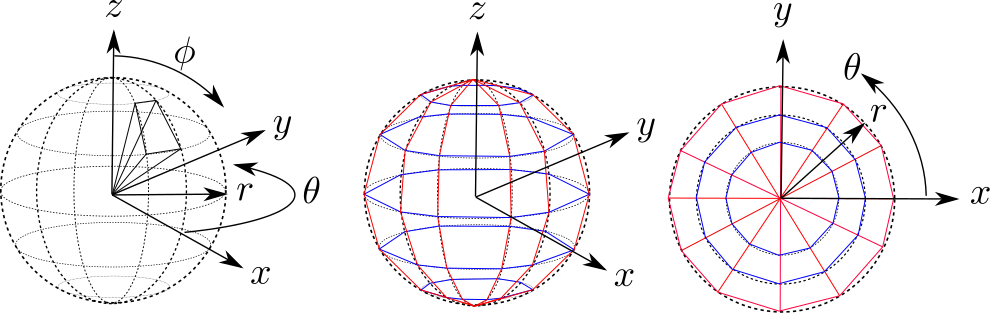
\includegraphics[scale=0.5]{Images//Coords//sph.png}
\caption[width=\columnwidth]{Diagram showing the meshing method for a spherical coordinate system\\
Red = Slices (12)\\
Blue = Stack (6)}
\label{sphmeshin}
\end{figure}

The meshing for the primitive solids in spherical coordinate systems are constructed by similar means the that of the spherical just with different trigonometric equations (\ref{trigsph}) as a result of two angle parameters $\phi$ and $\theta$. 
The trigonometry that converts the points from spherical coordinates to cartesian, are:

\begin{equation}
\begin{split}
x = r \cos{\theta}\sin{\phi}\\
y = r \sin{\theta}\sin{\phi} \\
z = z
\end{split}
\label{trigsph}
\end{equation}

\begin{lstlisting}[language=Python, caption=Python example]
for j0 in range(nslice):
    j1 = j0
    j2 = j0 + 1

    for i0 in range(nstack):
          i1 = i0
          i2 = i0 + 1
\end{lstlisting}



\subsubsection{Toroidal Co-ordinate System}
\begin{figure}[h!]
\centering
\includegraphics[scale=0.35]{Images//Coords/torus_coords.png}
\caption[width=\columnwidth]{Diagram showing the meshing method for a toroidal coordinate system}
\label{conts}
\end{figure}

The trigonometry that converts the points from toroidal coordinates to cartesian, are:

\begin{equation}
\begin{split}
x = R_{Torus} + R\cos{\theta}\cos{\phi} \\
y = R_{Torus} + R\cos{\theta}\sin{\phi} \\
z =  R\sin{\theta}
\end{split}
\end{equation}

\subsection{Plane Direction}
One key thing to be taken into account is the convention being used in the code for the order in which points are appended to make a plane, i.e to define a face on a solid. This is important as the direction the normal of the plane points in, dictates wether a face is considered an inside or outside face on the given solid. Getting this incorrect, will lead to missing faces, when the meshing is made. The concept is demonstrated in Figure \ref{pointsorder}.

\begin{figure}[h!]
\centering
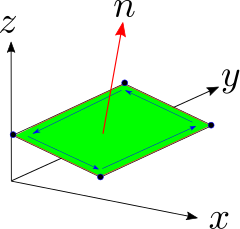
\includegraphics[scale=0.75]{Images//append_points//Point_Appending_Order.png}
\caption[width=\columnwidth]{Diagram showing the order convention of appending points to define the normal to a plane}
\label{pointsorder}
\end{figure}

\subsection{Degenerate points}


\subsection{Meshing performance testing}

\subsection{Curved primitive solids}
for each shape\\
stack and slice ?\\
radially mesh ?\\
which coord system

\newpage
\subsubsection{Cons}

\begin{figure}[h!]
\centering
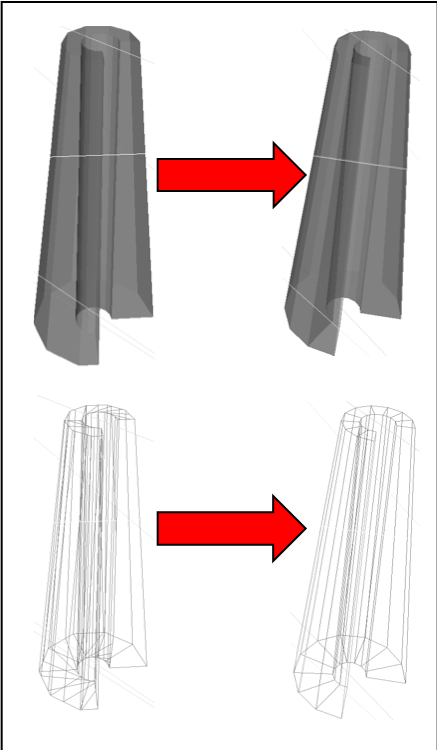
\includegraphics[scale=0.5]{Images//Meshes//cons.png}
\caption[width=\columnwidth]{Toroidal Coordinate System}
\label{conts}
\end{figure}

\begin{figure}[h!]
\centering
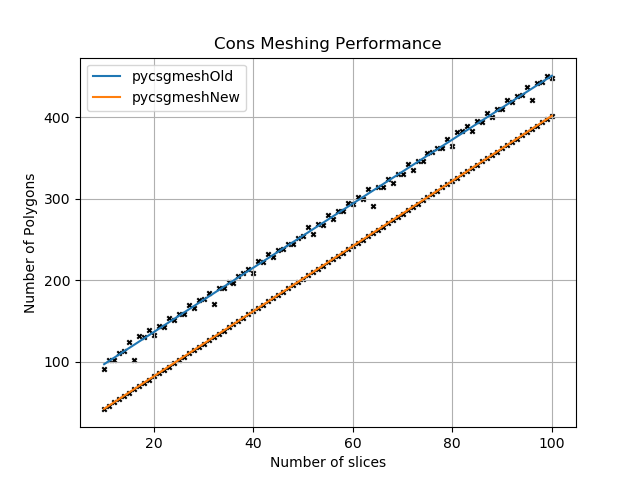
\includegraphics[scale=0.5]{Images//Quad_fits//Cons_quad.png}
\caption[width=\columnwidth]{Spherical Coordinate System}
\label{conts}
\end{figure}

\newpage
\subsubsection{CutTubs}

\begin{figure}[h!]
\centering
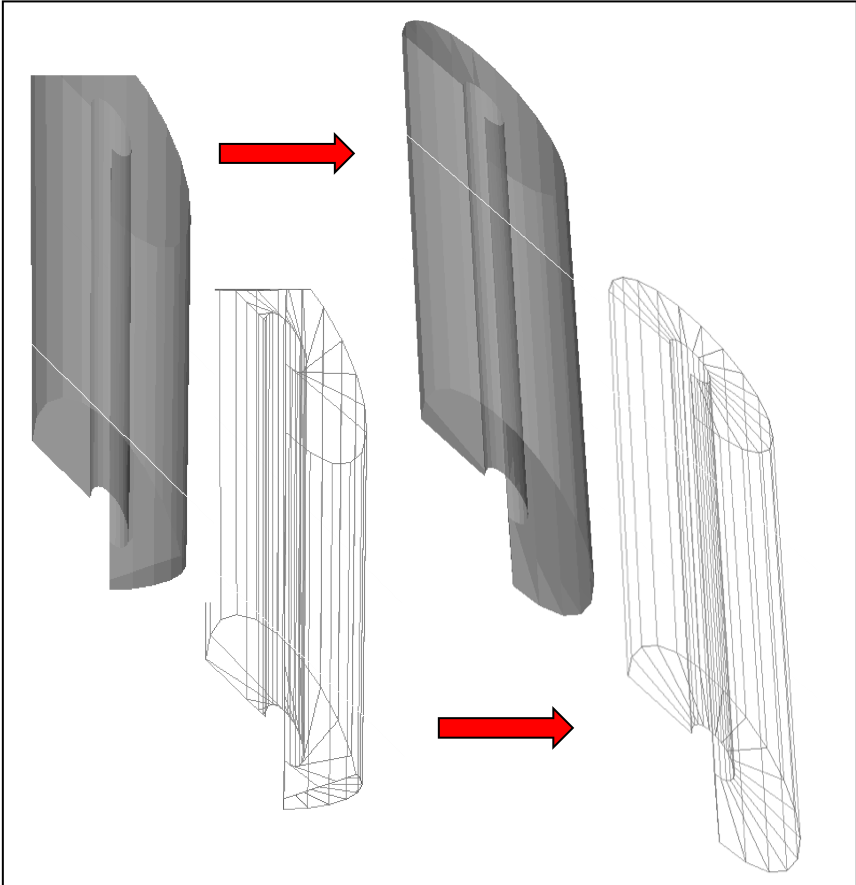
\includegraphics[scale=0.5]{Images//Meshes//CutTubs.png}
\caption[width=\columnwidth]{Toroidal Coordinate System}
\label{conts}
\end{figure}

\begin{figure}[h!]
\centering
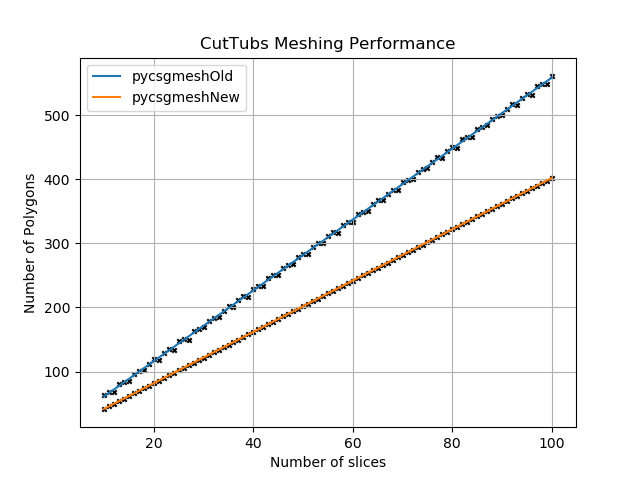
\includegraphics[scale=0.5]{Images//Quad_fits//CutTubs_quad.png}
\caption[width=\columnwidth]{Spherical Coordinate System}
\label{conts}
\end{figure}

\newpage
\subsubsection{Ellipsoid}

\begin{figure}[h!]
\centering
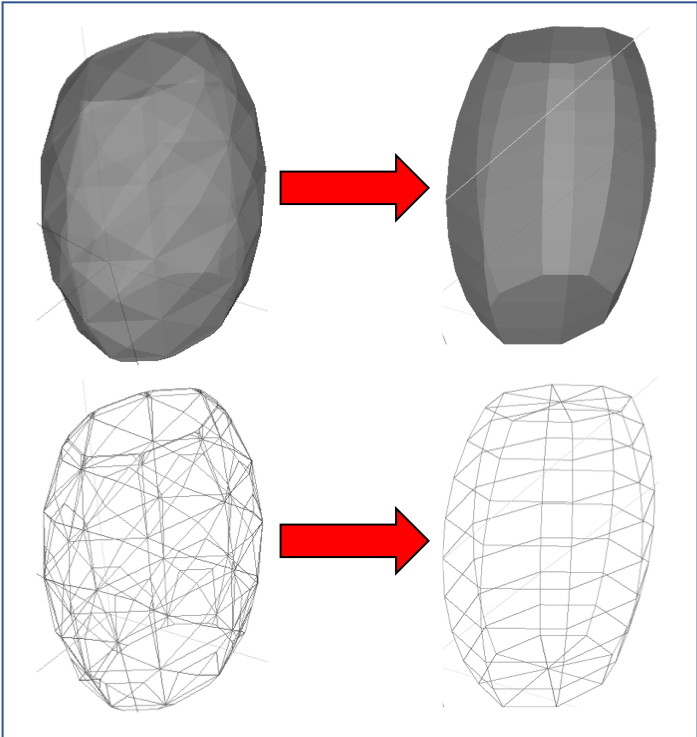
\includegraphics[scale=0.5]{Images//Meshes//ellipsoid.png}
\caption[width=\columnwidth]{Toroidal Coordinate System}
\label{conts}
\end{figure}

\begin{figure}[h!]
\centering
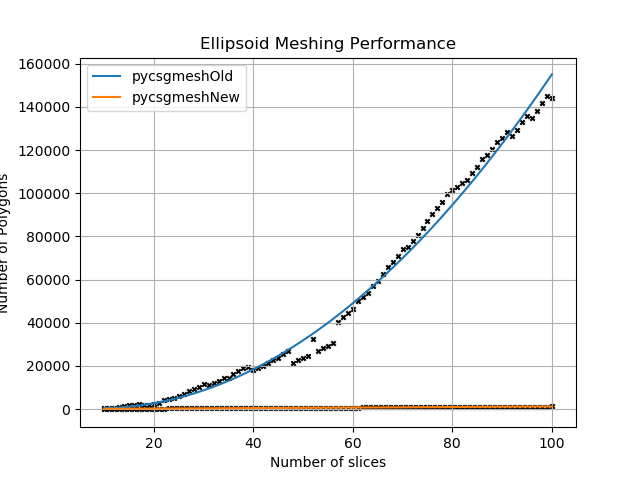
\includegraphics[scale=0.5]{Images//Quad_fits//Ellipsoid_quad.png}
\caption[width=\columnwidth]{Spherical Coordinate System}
\label{conts}
\end{figure}


\newpage
\subsubsection{EllipticalCone}

\begin{figure}[h!]
\centering
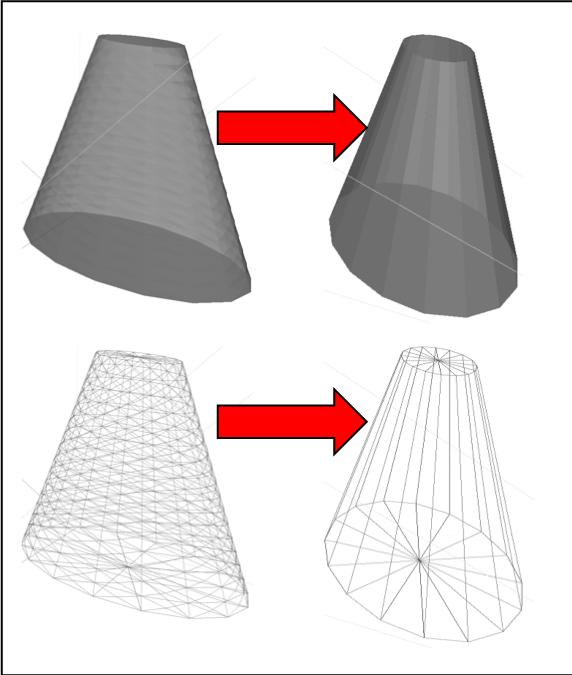
\includegraphics[scale=0.5]{Images//Meshes//ellipticalcone.png}
\caption[width=\columnwidth]{Toroidal Coordinate System}
\label{conts}
\end{figure}

\begin{figure}[h!]
\centering
\includegraphics[scale=0.5]{Images//Quad_fits//Ellipticalcone_quad.png}
\caption[width=\columnwidth]{Spherical Coordinate System}
\label{conts}
\end{figure}


\newpage
\subsubsection{EllipticalTube}

\begin{figure}[h!]
\centering
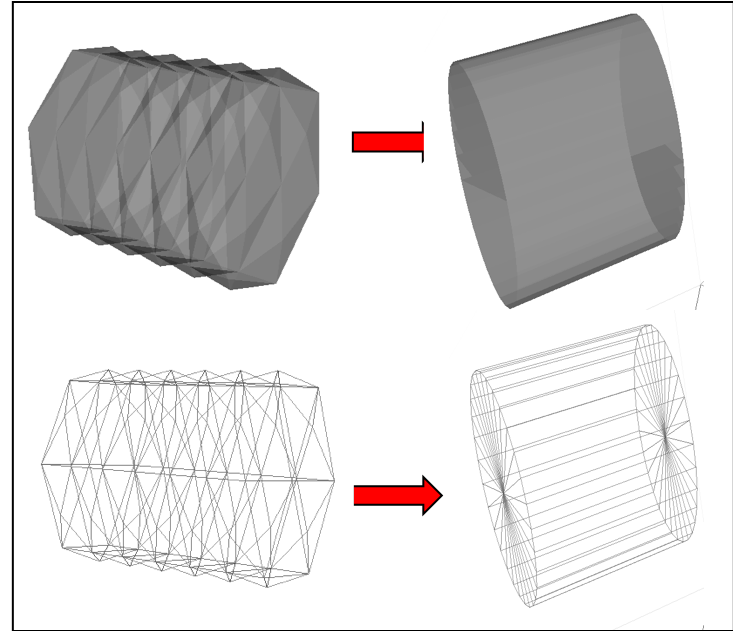
\includegraphics[scale=0.5]{Images//Meshes//ellipticaltube.png}
\caption[width=\columnwidth]{Toroidal Coordinate System}
\label{conts}
\end{figure}

\begin{figure}[h!]
\centering
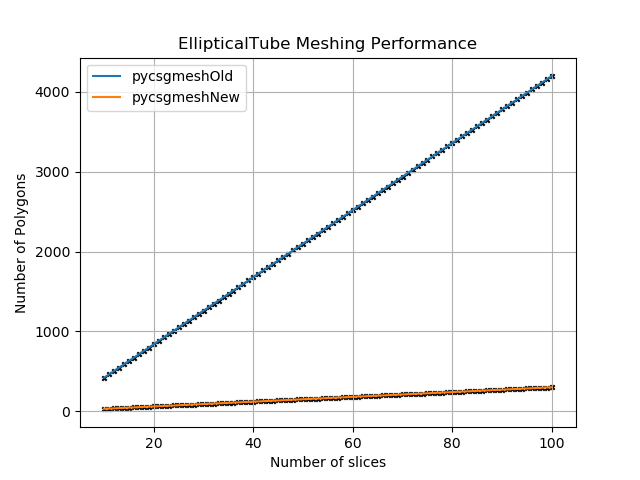
\includegraphics[scale=0.5]{Images//Quad_fits//EllipticalTube_quad.png}
\caption[width=\columnwidth]{Spherical Coordinate System}
\label{conts}
\end{figure}


\newpage
\subsubsection{Hyperboloid}

\begin{figure}[h!]
\centering
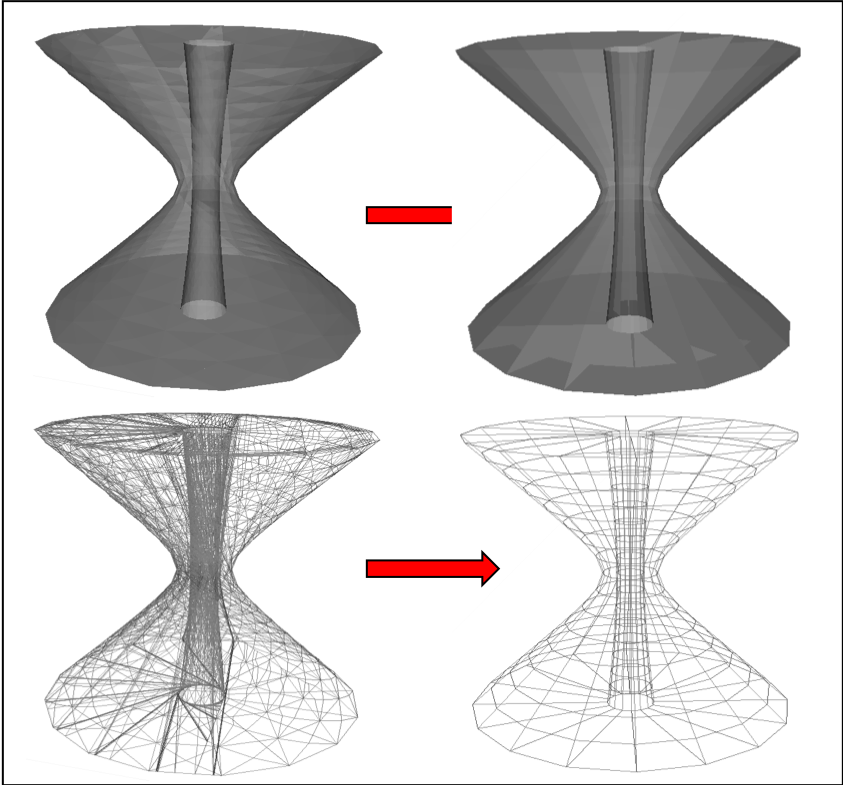
\includegraphics[scale=0.5]{Images//Meshes//hyperboloid.png}
\caption[width=\columnwidth]{Toroidal Coordinate System}
\label{conts}
\end{figure}


\newpage
\subsubsection{Orb}

\begin{figure}[h!]
\centering
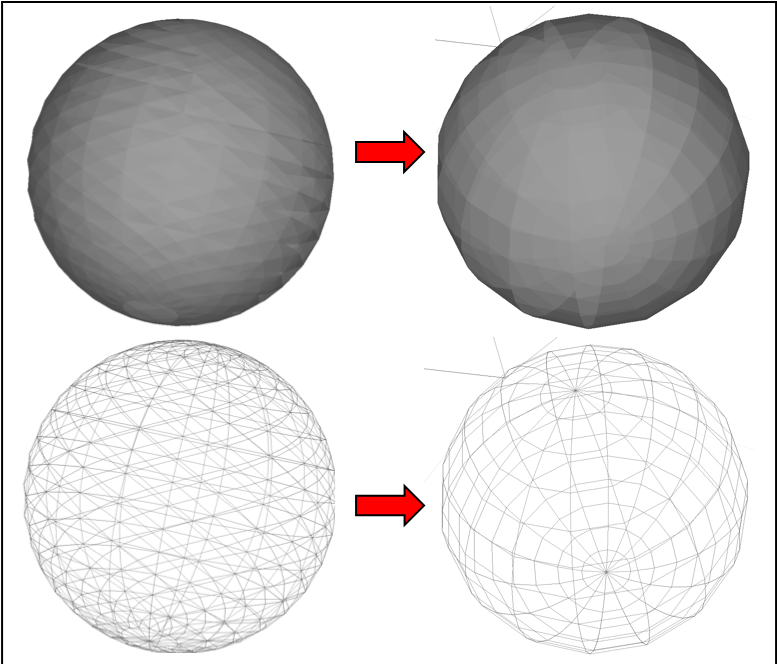
\includegraphics[scale=0.5]{Images//Meshes//orb.png}
\caption[width=\columnwidth]{Toroidal Coordinate System}
\label{conts}
\end{figure}

\begin{figure}[h!]
\centering
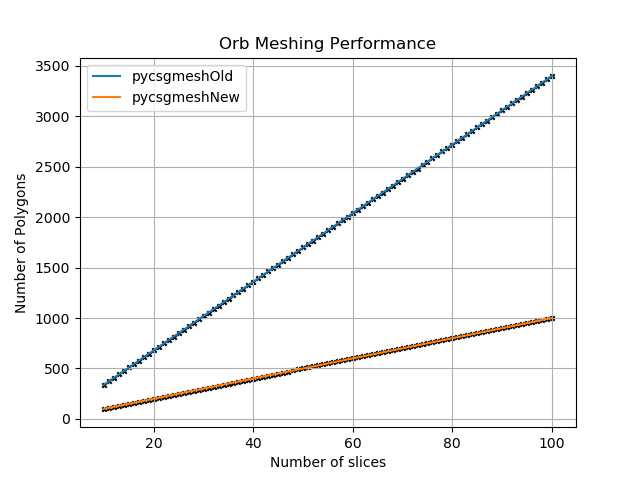
\includegraphics[scale=0.5]{Images//Quad_fits//Orb_quad.png}
\caption[width=\columnwidth]{Spherical Coordinate System}
\label{conts}
\end{figure}


\newpage
\subsubsection{Paraboloid}

\begin{figure}[h!]
\centering
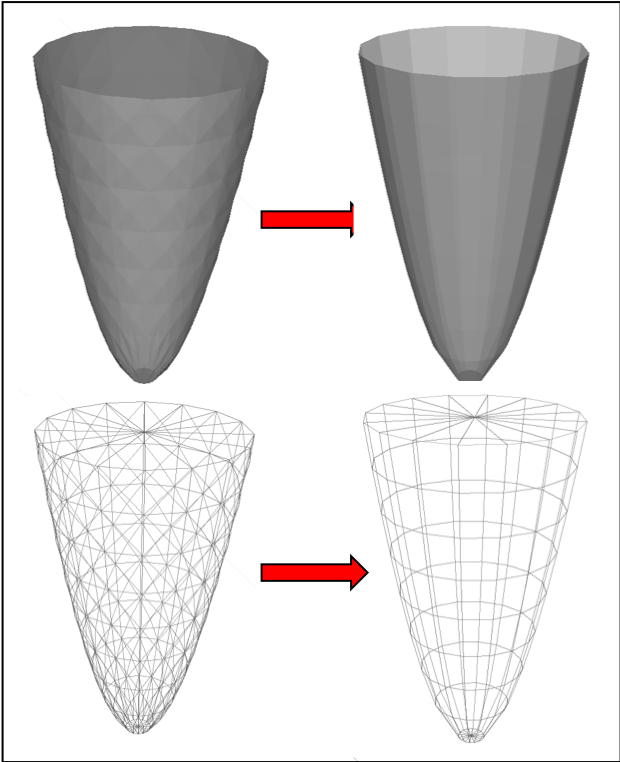
\includegraphics[scale=0.5]{Images//Meshes//paraboloid.png}
\caption[width=\columnwidth]{Toroidal Coordinate System}
\label{conts}
\end{figure}

\begin{figure}[h!]
\centering
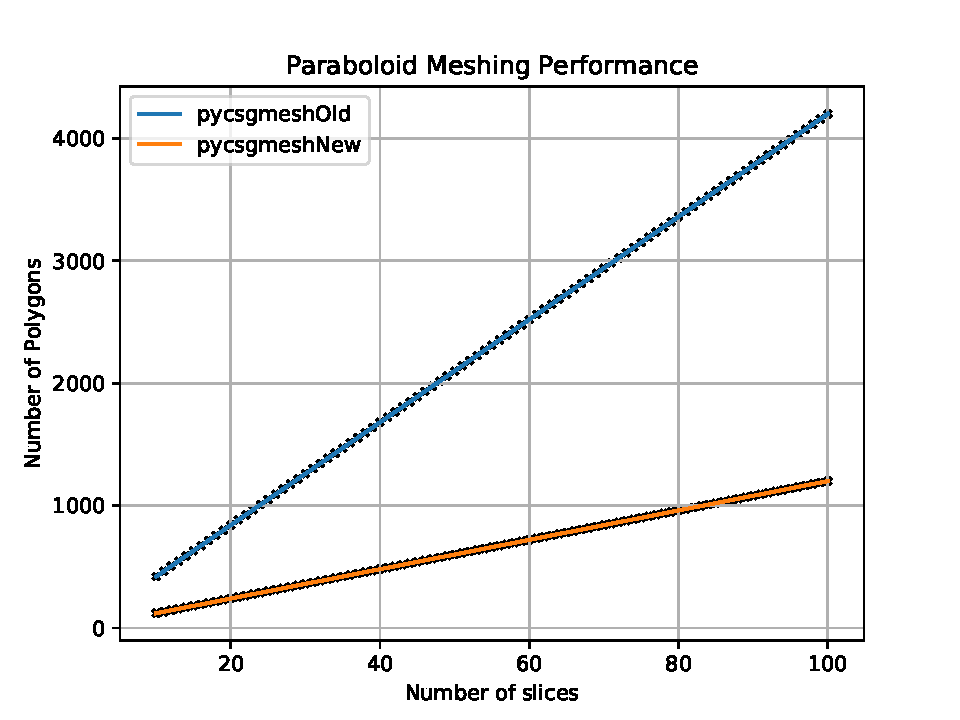
\includegraphics[scale=0.5]{Images//Quad_fits//Paraboloid_quad.png}
\caption[width=\columnwidth]{Spherical Coordinate System}
\label{conts}
\end{figure}


\newpage
\subsubsection{Polycone}

\begin{figure}[h!]
\centering
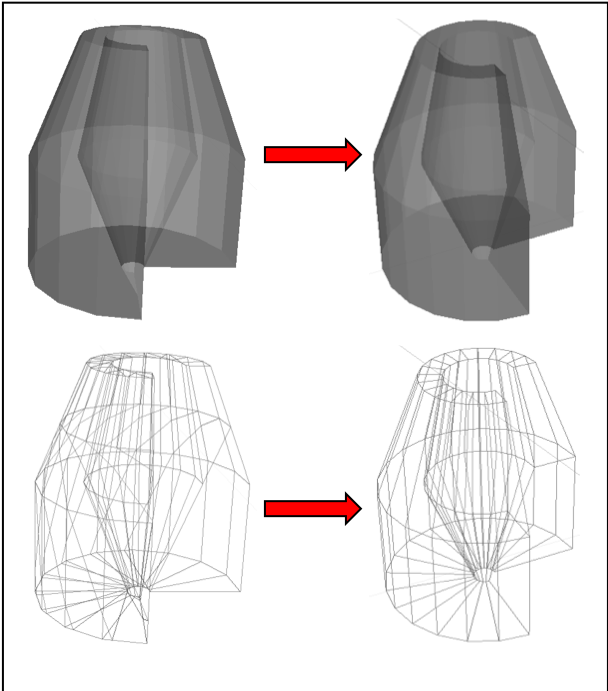
\includegraphics[scale=0.5]{Images//Meshes//polycone.png}
\caption[width=\columnwidth]{Toroidal Coordinate System}
\label{conts}
\end{figure}

\begin{figure}[h!]
\centering
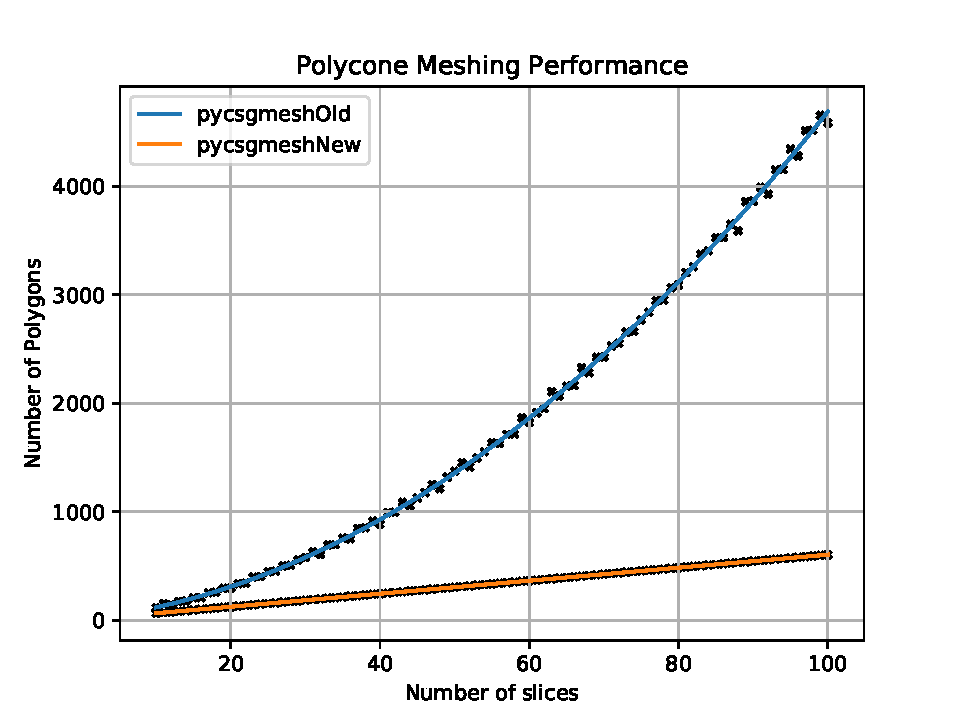
\includegraphics[scale=0.5]{Images//Quad_fits//Polycone_quad.png}
\caption[width=\columnwidth]{Spherical Coordinate System}
\label{conts}
\end{figure}


\newpage
\subsubsection{Sphere}

\begin{figure}[h!]
\centering
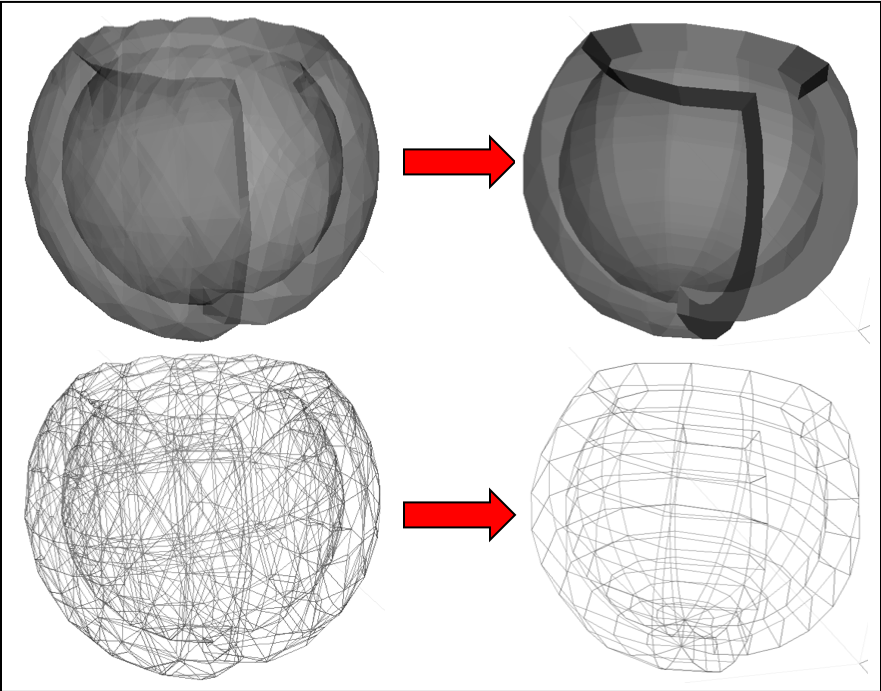
\includegraphics[scale=0.5]{Images//Meshes//sphere.png}
\caption[width=\columnwidth]{Toroidal Coordinate System}
\label{conts}
\end{figure}

\begin{figure}[h!]
\centering
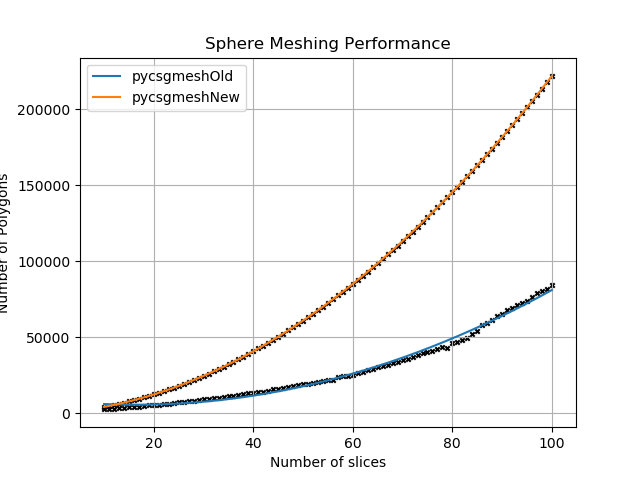
\includegraphics[scale=0.5]{Images//Quad_fits//Sphere_quad.png}
\caption[width=\columnwidth]{Spherical Coordinate System}
\label{conts}
\end{figure}


\newpage
\subsubsection{Torus}

\begin{figure}[h!]
\centering
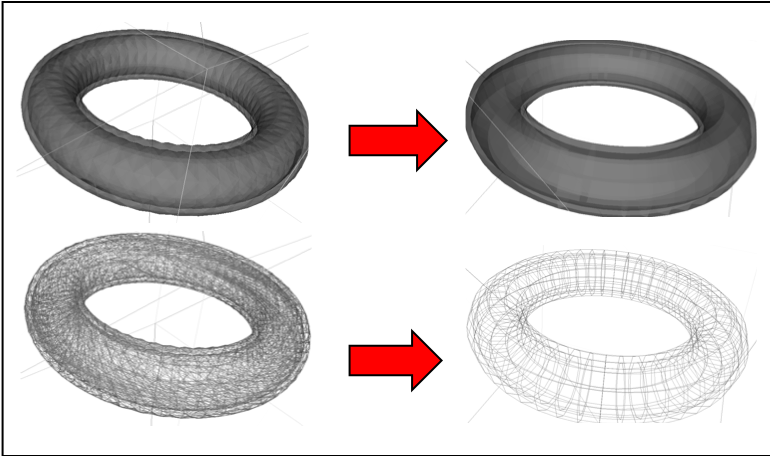
\includegraphics[scale=0.5]{Images//Meshes//torus.png}
\caption[width=\columnwidth]{Toroidal Coordinate System}
\label{conts}
\end{figure}

\begin{figure}[h!]
\centering
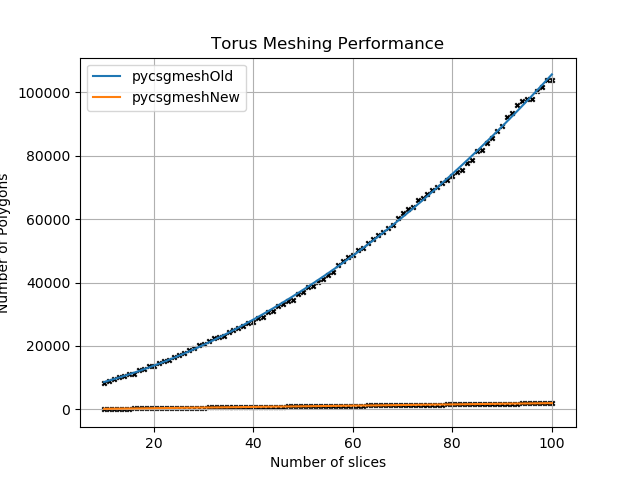
\includegraphics[scale=0.5]{Images//Quad_fits//Torus_quad.png}
\caption[width=\columnwidth]{Spherical Coordinate System}
\label{conts}
\end{figure}


\newpage
\subsubsection{Tubs}

\begin{figure}[h!]
\centering
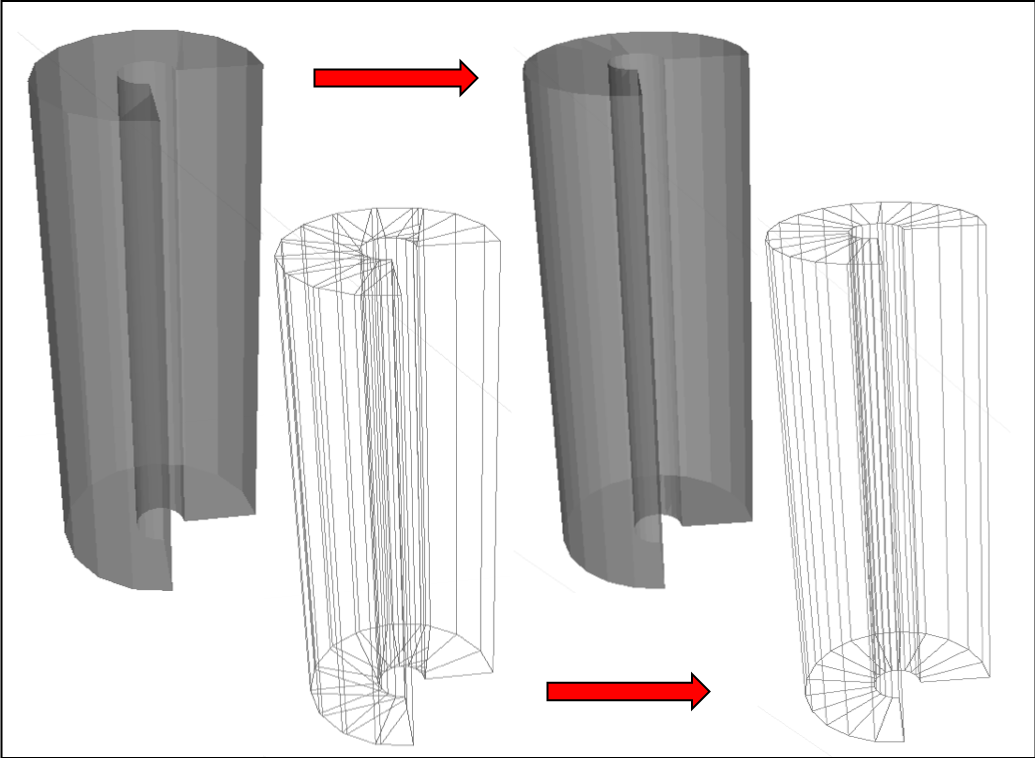
\includegraphics[scale=0.5]{Images//Meshes//tubs.png}
\caption[width=\columnwidth]{Toroidal Coordinate System}
\label{conts}
\end{figure}

\begin{figure}[h!]
\centering
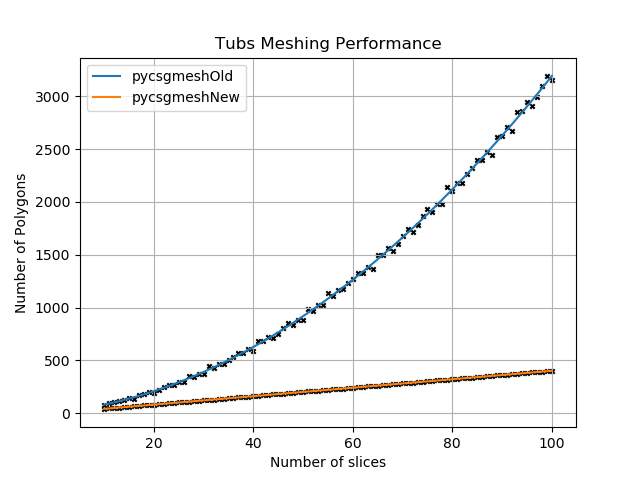
\includegraphics[scale=0.5]{Images//Quad_fits//Tubs_quad.png}
\caption[width=\columnwidth]{Spherical Coordinate System}
\label{conts}
\end{figure}

\newpage
\subsection{Performance tests}
table of perfrmance for each shape\\
plots\\

\section{BDSIM}
\subsection{Particle collisions with meshed solids}

\section{CAD}


 %%%%%%%%%%%%%%%%%%%%%%%%%%%%%%%%%%%%%%%%%%%%%%%%%%%%%%%%%%%%%%%%%%%%%%
 
\newpage

%\bibliographystyle{ieeetr}
%\bibliography{library}

\bibliographystyle{IEEEtran}
\bibliography{IEEEabrv,library}

\newpage
\section{Appendix (Python scripts)}
This section lists the Python scripts used to generate some of the figures within this report.
Data taken from Online NASA's confirmed exoplanet archive \cite{arch}, downloaded as .cvs file and imported into Python 3.7. ``path'' is the path to your ``.cvs'' type file. May be required to delete unnecessary rows explaining column headers.
%\appendix
%\subsection{Discoveries by year histogram (Figure \ref{hist})}\label{ap1}
%\lstinputlisting[language=Python]{Python//histogram.py}
%
%\newpage
%\subsection{Discovery method contribution pie chart (Figure \ref{pie})}\label{ap2}
%\lstinputlisting[language=Python]{Python//pi.py}

\end{document}